\documentclass{shureport}
% =============================================
% Part 0 Edit the info
% =============================================

\major{计算机科学与技术}
\name{王小明}
\title{实验报告}
\stuid{123456789}
\college{计算机工程与科学学院}
\date{\zhtoday}
\course{汇编语言程序设计}
\instructor{杨洪斌}
\expname{用表格形式显示字符}

\begin{document}
% =============================================
% Part 1 Header
% =============================================
\makecover


% =============================================
% Part 2 Main document
% =============================================

\section{实验目的}
通过循环控制编程方式用表格形式显示ASCII 字符表。
\section{实验要求}
按15 行×16 列的表格形式显示ASCII 码为10H—100H 的所有字符,即以行为主的顺序
及ASCII 码递增的次序显示对应的字符。每16 个字符为一行,每行中的相邻两个字符之间
用空白符(ASCII 为0)隔开。

\section{实验内容及思路}
    \subsection{实验内容}
    本次实验的主要内容为按15行每列16个ASCII 码以表格形式显示这些ASCII码。
    \subsection{实验思路}
    对于这个实验,我们可以将实验过程分为如下两大步骤:
    %% 这里也可以使用 `subsubsection`
        \begin{enumerate}
            \item 计算出10H-100H的值,并将其置入寄存器中
            \item 将上述寄存器的值输出到屏幕上 
        \end{enumerate}

\section{实验步骤}
        \subsection{编写汇编代码}
            \begin{enumerate}
                \item 计算ASCII码的值
                \par 由于我们最终要以15行每列16个ASCII码的表格形式程序实验结果,所以我们很容易就想到了用
                双重循环来计算ASCII码的值。外层循环为15次,用于计算行值;内层循环为16次,用于计算列值。
                需要注意的是,在内层循环中,每输出一个ASCII码值,就要输出一个空格(ASCII码值为0),在两个
                外层循环间还要输出一个换行和一个回车。
                \item 输出部分
                \par DOS系统21号中断的2号功能($AH=02$)可以将一个字符显示输出,因此,我们只需将21号中断的2号功能
                封装成一个函数,每次输出字符时调用该函数即可。
            \end{enumerate}
        \subsection{编译链接并执行}
            \begin{enumerate}
                \item 打开DOSBox,挂载相应目录
                \item 键入 masm ascii.asm,回车
                \item 键入 link assii.obj,回车
                \item 键入 assii.exe,回车
            \end{enumerate}


\section{实验代码及结果}
    \subsection{实验代码}
    实验代码如下:
        \lstinputlisting[language={[x86masm]Assembler}]{code/ascone.asm}
    
    \subsection{实验结果}
    实验结果如图~\ref{fig:ascii} 所示。
        \begin{figure}[!htbp]
            \centering
            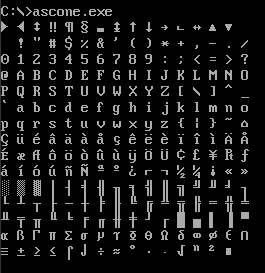
\includegraphics[width=0.6\linewidth]{ascii.png}
            \caption{ASCII码为10H-100H的所有字符}
            \label{fig:ascii}
        \end{figure}

\section{实验体会}
本次实验最大的收获是对call和ret的原理有了更深刻的理解。开始时我认为call和ret会自动对所有寄存器的值做压栈和出栈操作。但在
本次实验中,我发现,如果在call一个函数之后系统不会对通用寄存器的值进行压栈操作,通用寄存器的值将在函数调用过程中将发生改变。进过查阅课本
我发现,call和ret在调用函数过程中,仅对程序在调用函数时的下一地址进行压栈出栈操作,这纠正了我之前的错误认识。
\end{document}
